
\documentclass[12pt,oneside]{memoir}

\usepackage{matfmaster}


\usepackage{cmsrb}


\usepackage{listings}
\usepackage{color}
\definecolor{lightgray}{rgb}{.9,.9,.9}
\definecolor{darkgray}{rgb}{.4,.4,.4}
\definecolor{purple}{rgb}{0.65, 0.12, 0.82}
\lstdefinelanguage{JavaScript}{
  keywords={break, case, catch, continue, debugger, default, delete, do, else, false, finally, for, function, if, in, instanceof, new, null, return, switch, this, throw, true, try, typeof, var, void, while, with, test, await, async, let, const, expect, forEach, toBe, import, render},
  morecomment=[l]{//},
  morecomment=[s]{/*}{*/},
  morestring=[b]',
  morestring=[b]",
  keywordstyle=\color{blue}\bfseries,
  ndkeywordstyle=\color{darkgray}\bfseries,
  identifierstyle=\color{black},
  commentstyle=\color{purple}\ttfamily,
  stringstyle=\color{red}\ttfamily,
  sensitive=true
}

\lstset{
   language=JavaScript,
   backgroundcolor=\color{white},
   extendedchars=true,
   basicstyle=\footnotesize\ttfamily,
   showstringspaces=false,
   showspaces=false,
   numbers=left,
   numberstyle=\footnotesize,
   numbersep=9pt,
   tabsize=2,
   breaklines=true,
   showtabs=false,
   captionpos=b
}
\bib{literatura}

\autor{Никола Димић}
% Naslov teze na srpskom jeziku (u odabranom pismu)
\naslov{Аутоматстко тестирање микросервисних апликација}
% Godina u kojoj je teza predana komisiji
\godina{2022}
% Ime i afilijacija mentora (u odabranom pismu)
\mentor{др Милена \textsc{Вујошевић Јаничић}, ванредни професор\\ Универзитет у Београду, Математички факултет}
% Ime i afilijacija prvog člana komisije (u odabranom pismu)
\komisijaA{др Саша \textsc{Малков}, ванредни професор\\ Универзитет у Београду, Математички факултет}
% Ime i afilijacija drugog člana komisije (u odabranom pismu)
\komisijaB{др Филип \textsc{Марић}, ванредни професор\\ Универзитет у Београду, Математички факултет}
% Ime i afilijacija trećeg člana komisije (opciono)
% \komisijaC{}
% Ime i afilijacija četvrtog člana komisije (opciono)
% \komisijaD{}
% Datum odbrane (obrisati ili iskomentarisati narednu liniju ako datum odbrane nije poznat)
\datumodbrane{септембар 2022.}

% Apstrakt na srpskom jeziku (u odabranom pismu)
\apstr{ Микросервисна архитектура представља популарно решење за дизајнирање комплексних дистрибуираних система. Аутоматизацијом тестирања микросервисних система може се осигурати велика поузданост како појединачних сервиса тако и целокупног система. Циљ рада представља сагледавање особина микросервисне архитектуре, као и техника аутоматског тестирања које се могу применити на систем који ту архитектуру користи. У склопу рада је развијена једноставна микросервисна веб апликација \textit{Gelos} и оквир за аутоматско тестирање те апликације на више нивоа.
}

% Ključne reči na srpskom jeziku (u odabranom pismu)
\kljucnereci{развој софтвера, верификација софтвера, аутоматско тестирање, микросервиси, развојни оквир \textit{Playwright}}
\begin{document}
% ==============================================================================
% Uvodni deo teze
\frontmatter
% ==============================================================================
% Naslovna strana
\naslovna
\komisija
\posveta{
Захваљујем се менторки на саветима и подршци и родитељима, сестри и Нади на помоћи и мотивацији.
}
% Strana sa podacima o disertaciji na srpskom jeziku
\apstrakt
% Sadržaj teze
\tableofcontents*

% ==============================================================================
% Glavni deo teze
\mainmatter
% ==============================================================================

% ------------------------------------------------------------------------------
\chapter{Увод}
% ------------------------------------------------------------------------------

Микросервисна архитектура постала jе популаран избор дизаjна апликациjа услед добре скалабилности решења, минималне спреге делова система и могућности брзог развоjа софтвера. Интеграциjа постоjећих микросервиса у склопу имплементациjе софтверских решења и брз развоj додатно повећаваjу важност тестирања.
Аутоматизациjа тестирања значајно  убрзава процес имплементациjе и повећава поузданост софтверског решења, али представља велики изазов поготово у дистрибуираним системима. Циљ овог рада је опис карактеристика микросервисне архитектуре и начина на који се технике аутоматског тестирања могу применити на апликацију која користи ту архитектуру.

У оквиру рада имплементирана је микросервисна апликација ,,\textit{Gelos}” која за циљ има претраживање и помоћ при избору филма односно књиге за читање, након чега је имплементиран систем за тестирање те апликације на више нивоа. Систем који се тестира састоји се од два микросервиса и клијентске апликације. Кроз јединичне, интеграционе и системске тестове представљене су могућности аутоматизације тестова овог система у целости.

У поглављу \ref{chp:mikroservisi} представљене су карактеристике и особине које одликују микросервисну архитектуру. Поред тога направљен је осврт на начине интеграција сервиса, кроз дефинисање архитектуре \textit{REST} (енг. \textit{REpresentational State Transfer}). Поглавље се такође бави архитектуралним решењима за имплементацију појединачних микросервиса.

Поглавље \ref{chp:testiranje} обрађује тему аутоматског тестирања. Дефинисањем различитих модела за поделу тестова представљени су различити начини и типови тестирања, уз осврт на примену тих типова на микросервисне апликације. У склопу поглавља посвећена је пажња и архитектуралним решењима за систем тестирања као што је\textit{ Модел странице као објекта} (енг. \textit{Page Object Model})

Поглавље \ref{chp:aplikacija} укратко даје преглед технологија употребљених приликом имплементације апликације и система за тестирање. Такође, поглавље описује начин креирања сваког од микросервиса, као и клијентске апликације. Након тога представља начин имплементације јединичних, интеграционих и системских тестова који су одговорни за поузданост апликације.

 У последњем, \ref{chp:zakljucak}. поглављу, изведен је закључак где су сумирани доприноси и начини за даља унапређења.



% ------------------------------------------------------------------------------
\chapter{Микросервисна архитектура}
\label{chp:mikroservisi}
% ------------------------------------------------------------------------------

Усложњавањем проблема који се решавају софтверским решењима расте и комплексност апликације која тај проблем решава. Као и код многих математичких проблема, комплексност у софтверским решењима превазилази се разбијањем домена проблема у више поддомена. 

При коришћењу монолитне архитектуре проблем комплексности решења решава се техникама које теже ка што већој кохезивности кода. Кохезивност кода представља идеју груписања модула сличних функционалности заједно. 
Микросервисна архитектура такође почива на овом принципу, али је циљ комплетно раздвајање делова система уз јасно дефинисане границе. 

Микросервисна архитектура представља архитектурални стил који структуира систем као скуп малих сервиса који су минимално спрегнути, оријентисани ка специфичном домену, и лаки за интеграцију и одржавање. Сваки сервис представља логичку целину која је минимално спрегнута у односу на остале делове система.

Како би се лако интегрисао, сервис дефинише јавни интерфејс преко ког може комуницирати са другим сервисима. Комуникација између сервиса најчешће се одвија путем мрежних позива, који представљају скупе операције, па је ниска спрегнутост приликом пројектовања система подразумевана. 

% Da li pricati o monolitnoj ?

 \newpage

\section{Особине архитектуре}

Предности и мане микросервисне архитектуре већински проистичу из особине ниске спрегнутости делова система. Велика сличност са дистрибуираним системима подразумева сличне дилеме приликом одабира микросервисне архитектуре као софтверског решења.

Неке од особина архитектуре су композитност, отпорност на отказивање, лако скалирање, локализовање података, технолошка хетерогеност и могућност дистрибуирања послова. Ипак микросервисна архитектура не представља универзално софтверско решење, па је не треба користити у свим ситуацијама \cite{microservicesBook}. У наставку поглавља биће детаљније речи о поменутим особинама микросервисне архитектуре уз осврт на разлике у односу на монолитну архитектуру. 

Због раздвојености делова система и ниског нивоа стандардизације интерфејса, детектовање грешака унутар система представља велики изазов приликом имплементације микросервисних апликација. Tема тестирања микросервисних апликација биће детаљно обрађена у поглављу \ref{chp:testiranje}.

\subsection{Композитност}

Одвајањем логичких компоненти које су одговорне за специфичан део апликације, омогућава се смањење редундантности кода и коришћење постојећих решења при имплементацији. Сличне апликације често имају заједнички подскуп функционалности. Како је путем интерфејса једноставно повезати више сервиса, већ постојећи сервиси се лако могу укомпоновати при имплементацији новог система \cite{microservicesBook}. 

За проблеме који су врло чести, попут ауторизације и аутентификације унутар апликације, постоји велики број постојећих микросервисних решења која се једноставно могу интегрисати у микросервисну апликацију. Уколико одређени сервис не задовољава захтеве апликације може се заменити уз минималне измене кода.

\subsection{Дистрибуирање развоја и технолошка хетерогеност}

Ниска спрегнутост омогућава паралелни развој делова система, али и могућност коришћења различитих технолошких и архитектуралних решења за сваки од микросервиса. Tимови могу паралелно радити на различитим целинама система имплементирајући унапред договорен јавни интерфејс сервиса. Сваки сервис кроз свој интерфејс дефинише који ће део система бити доступан кориснику.

Променама унутар појединачних сервиса не мења се целокупан рад система, све док су интерфејси непромењени. У односу на перформансе које су захтеване, сваки микросервис може користити ону врсту базе података, радног оквира или програмског језика који најбоље одговара проблему који сервис решава. Експериментисање са новим технологијама има знатно мање последице по целокупан рад система јер се промене изолују само на један микросервис, за разлику од монолитних система, где промене у технолошком домену подразумевају мењање целокупног система \cite{microservicesBook}.


\subsection{Локализовање података}

Како би сервис био комплетно одговоран за специфичан посао, потребно је да буде независан и на нивоу података. Сваки микросервис користи сопствену колекцију података или податке добија од других сервиса који имају специфичну намену. Независност на нивоу података омогућава преносивост и вишеструку употребљивост али и отежава пројектовање због повећане опасности од редундантости.


\subsection{Скалирање}

Услед повећања броја корисника апликације потребно је повећати хардверске ресурсе додељене систему. Коришћењем монолитне архитектуре ово представља велики изазов јер је овакав тип скалирања могућ само уколико се целокупан систем скалира. С друге стране, микросервисна архитектура омогућава повећавање хардверских ресурса само за оне делове система којима је то неопходно. Скалирање се може обављати и динамички тако што ће се сервису, на основу броја захтева, доделити одговарајући ресурси \cite{microservicesBook}.


\subsection{Отпорност на отказивање}

Отказивање делова система код монолитних апликација подразумева пад комплетне апликације. Монолитне апликације превазилазе тај проблем покретањем апликације на више инстанци како би се смањила вероватноћа отказа целог система. Ова метода захтева додатне ресурсе и комплексан систем који регулише апликацију у случају пада.

Насупрот томе, пад једног од делова микросервисне апликације не утиче на рад остатка система. Уколико постоји резервна инстанца сервиса који је отказао, апликација може наставити са нормалним функционисањем. Ако то није случај, апликација може наставити да ради са редукованим функционалностима.


\subsection{Брзо испоручивање софтвера}

Непрекидно испоручивање софтвера (енг. \textit{continuous deployment}) један је од централних принципа агилног развоја софтвера. Испоручивање софтвера дефинисано је као низ корака које је потребно одрадити како би се нова верзија апликације оспособила за употребу. Овај процес састоји се од корака као што су дистрибуција нове верзије, инсталација, деинсталација, ажурирање и праћење верзија.

При коришћењу монолитне апликације, свака промена у коду најчешће захтева да се цела апликација испоручи. Како је испорука комплексан процес, у пракси се испоручивање софтвера врши тек када је одређен скуп промена извршен. Увећавањем скупа измена у коду, расте и шанса да ће приликом испоруке софтвера доћи до грешке. Услед великог броја измена, наћи конкретну промену која је довела до грешке може бити захтевно и временски скупо. 

Микросервисна архитектура омогућава да се промене на једном микросервису испоручују независно од остатка система. Уколико се испорука не изврши исправно, налажење грешке знатно је једноставније јер је изоловано на један део система, док остали остају непромењени. Дистрибуирање нових верзија кода се извршава брже јер се пре испоруке не морају чекати остали делови система. Међутим, раздвајање испоручивања софтвера за сваки од сервиса није без последица. Како би апликација користила најновије стабилне верзије кода, потребно је имплементирати специфичан систем за испоручивање софтвера у зависности од апликације \cite{microservicesBook}. Овај систем често може бити јако комплексан па захтева детаљно планирање при дизајнирању.

\newpage

\section{Интеграција микросервиса}

Начин комуникације између сервиса представља јако битан аспект пројектовања микросервисне апликације. Исправно дизајниран начин комуникације треба да омогући сервисима да кроз развој задрже своју aутономност и да се мењају независно од остатка система. 

Тежећи ка једноставним и брзим начинима интеграције сервиса, микросервисна архитектура се одликује одсуством строге формализације протокола. У наставку поглавља биће речи о једном од једноставнијих, и баш из тог разлога, популарнијих начина интегрисања микросервиса  --- коришћењем обрасца архитектуре \textit{REST}  у комбинацији са \textit{HTTP} протоколом.

\subsection{Образац архитектуре \textit{REST} и \textit{HTTP} протокол}

Образац архитектуре \textit{REST} (енг. \textit{REpresentational State Transfer}) представља скуп принципа и ограничења помоћу којих системи могу комуницирати. Принципи архитектуре који омогућавају лаку интеграцију микросервиса су:

\begin{description}
\item[Клијент - сервер]  --- архитектура је заснована на Вебу па подразумева раздвајање клијентског и серверског дела система. Све док је интерфејс стандардизован, клијентски и серверски део система се могу независно развијати. Раздвајање система на микросервисе представља уопштење овог принципа.
\item[Без стања] --- архитектура подразумева да сваки клијентски захтев ка серверу мора садржати све потребне информације без обзира на тренутно стање сервера. Сервер не чува информације о тренутној сесији између клијента и сервера. Уопштено на микросервисну архитектуру, ни један од сервиса не чува информације о комуникацији са клијентом или другим сервисом.
\item[Ресурси] --- архитектура као централну аутономну јединицу поставља ресурс. Ресурси представљају податке којима сервис располаже. Начин на који сервис интерно манипулише подацима сакривен је од корисника. Репрезентација у којој се подаци шаљу кориснику зависи од клијентског захтева и стога се репрезентација ресурса може мењати.
\end{description}

Стандардизација интерфејса, односно порука које се шаљу између сервиса, захтева добро дефинисан протокол. При имплементацији \textit{REST} архитектуре могуће је користити различите протоколе, али се у пракси најчешће користи \textit{HTTP}.

\textit{HTTP} (енг. \textit{HyperText Transfer Protocol}) протокол користи скуп метода помоћу којих је могуће оперисати подацима, као што су \textit{GET}, \textit{POST}, \textit{PUT} и \textit{DELETE}.  Уместо креирања посебних функција за манипулацију ресурсима, могу се користити постојеће методе које протокол већ пружа. Како је ресурс централна јединица архитектуре, свака од ових метода има јасно значење: 
\begin{itemize}
\item \textit{GET} --- дохвата ресурс,
\item \textit{POST} --- креира ресурс,
\item \textit{PUT} --- ажурира ресурс,
\item \textit{DELETE} --- брише ресурс.
\end{itemize}

Помоћу дефинисаних метода шаљу се захтеви ка серверу или сервису. Протокол дефинише и формат одговора на послате захтеве. У сваком одговору налази се информација о статусу извршене операције у форми статусног кода. Сваки од кодова има семантичко значење, па тако код \textit{200} значи да је операција успешно завршена, док код \textit{404} обавештава корисника да ресурс није пронађен. Осим статусних кодова, одговор може садржати податке као што су репрезентације ресурса или метаподатке попут броја ресурса којима се може приступити.

\newpage
\section{Дизајн микросервиса}

Микросервисна архитектура омогућава коришћење различитих архитектуралних решења приликом имплементације микросервиса. Архитектурални стил сваког микросервиса мора да подржава раздвајање одговорности од остатка апликације. Један од образаца архитектуре коришћених за пројектовање микросервиса јесте архитектура Модел-Поглед-Контролер (енг.\textit{ Model-View-Controller, MVC}) о којој ће бити речи у наставку поглавља.

\subsection{Образац архитектуре Модел-Поглед-Контролер}

Образац архитектуре Модел-Поглед-Контролер заснива се на подели система на три целине, које имају различите функције.
\begin{description}
\item[Модел]представља структуру података.
\item[Поглед]представља приказ података у корисничком окружењу.
\item[Контролер]представља начин управљања подацима модела.
\end{description}

У контексту микросервиса, модел представља структуру података коју микросервис користи, што је најчешће база података. Контролер имплементира бизнис логику самог сервиса, односно управља подацима модела. Традиционално, када је у питању примена \textit{MVC} архитектуре на веб апликације, поглед представља приказ података у корисничком окружењу. Међутим, при имплементацији микросервиса, поглед представља јавни интерфејс, тј. оно што је изложено кориснику сервиса на коришћење. Раздвојеност делова омогућава паралелан рад на деловима сервиса, као и лакше измене унутар целина, попут замене базе података. 
% Проширити ?



% ------------------------------------------------------------------------------
\chapter{Аутоматско тестирање софтвера}
\label{chp:testiranje}
% ------------------------------------------------------------------------------

Тестирање софтвера представља процес провере софтвера са циљем проналажења грешака и провере квалитета. Процес тестирања проверава да ли су испуњени претходно дефинисани функционални и нефункционални захтеви \cite{ISTQB}.

Тестирање софтвера може потврдити постојање грешака у систему, али не може потврдити њихово одсуство. Самим тим, битно је тестирати што је више и чешће могуће како би поузданост система била већа. Ипак, није могуће све тестирати, услед експоненцијалног броја улазних вредности које треба проверити, како би сваки могући случај употребе био покривен. Како би се доступни ресурси искористили на најбољи могући начин, треба бирати шта и када се тестира. Аутоматско тестирање представља технику која значајно убзава процес верификације софтвера и самим тим омогућава да се већи број функционалности тестира.

Препорука је почети са тестирањем што раније у процесу развоја софтвера. Проналажење грешака у систему у каснијим фазама развоја има огроман утицај на квалитет софтвера јер се те грешке по правилу тешко отклањају. Константним тестирањем, чак и пре самог процеса имплементације софтвера, минимизују се грешке у касним фазама развоја. Процес аутоматизације значајно олакшава константне провере система и омогућава поновљив начин за тестирање развијених функционалности.


\section{Категоризација и начини тестирања}

Аутоматско тестирање представља технику тестирања која користи специјалне алате како би извршила проверу исправног извршавања теста. Насупрот томе, мануелно тестирање извшава особа не користећи ову врсту алата. Поставља се питање које тестове је могуће и како аутоматизовати.

Како би се исправно приступило проблему аутоматизације потребно је разумети различите категорије тестова као и циљеве тестирања које они имају. Категоризација тестова дефинисана је квадратом тестирања Брајана Марика приказаног на слици \ref{fig:kvadrat} \cite{testiranjeBook}. У доњем делу квадрата налазе се тестови који су окренути технологијама, односно помажу програмерима при имплементацији система. Аналогно, у горњем делу квадрата налазе се тестови који су окренути бизнис логици система, односно проверавају да ли систем задовољава захтеве корисника \cite{microservicesBook}. Посматрајмо сваку од категорија појединачно.

\begin{description}
\item[Тестови прихватања (енг. \textit{acceptance tests})]
\footnote{Тестови прихватања разликују се од корисничких тестова прихватања (енг. \textit{user acceptance tests}), који представљају врсту мануелног тестирања које извршавају реални корисници апликације. Како је циљ ове врсте тестова кориснички дојам о функционалностима апликације, ова врста тестова не може се аутоматизовати па није обрађена у склопу овог рада.}
--- проверавају да ли је имплементирана функционалност  одговара дефинисаним захтевима. Како ова врста тестова има јасно дефинисане захтеве односно улазне вредности и очекиване излазе за те вредности, погодни су за аутоматизацију. Представљају подршку процесу имплементације.

\item[Тестови истраживања (енг. \textit{exploratory tests})] --- проверавају да ли је могуће покварити неки део система коришћењем апликације. Како би овај тип тестирања био ефективан потребно је деструктивно приступити извршавању теста. Ово се најбоље постиже коришћењем интуиције приликом тестирања, па се овај вид тестова најчешће извршава мануелно.

\item[Јединични тестови (енг. \textit{unit tests})] --- проверавају да ли имплементирана функционалност исправно функционише. Услед малог скупа провера које је потребно извршити, ови тестови се углавном аутоматизују и представљају најосновнији али и најбржи вид аутоматских тестова.

\item[Тестови перформанси и безбедности (енг. \textit{performance and security tests})]  --- проверавају да ли систем испуњава очекиване перформансе, као што је време првог учитавања странице. Тестови безбедности проверавају у којој мери је систем заштићен од малициозних напада. Аутоматизовањем тестова перформанси проверава се у којој је мери систем оптимизован.
\end{description}



\begin{figure}[!ht]
  \centering
  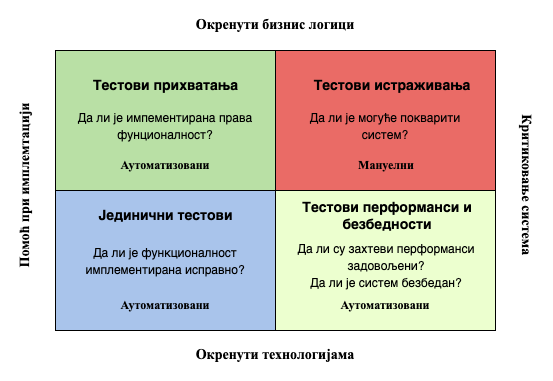
\includegraphics[width=0.8\textwidth]{matfmaster/img/kvadrat.png}
  \caption{Kвадрат тестирања Брајана Марика}
  \label{fig:kvadrat}
\end{figure}

Основни услов за аутоматизацију теста јесте детерминистичко понашање функционалности која се тестира. У пракси није могуће, а ни пожељно све аутоматизовати. Мануелно тестирање има предности за одређене типове тестирања али већински се тежи ка што већем нивоу аутоматизације. Како се систем мења тако је потребно мењати и аутоматске тестове који га тестирају. Приликом додавања нових функционалности битно је паралелно додавати нове аутоматске тестове, како би поузданост система остала иста. Време извршавања теста као и број тестова варирају у зависности од типа теста. У наставку биће приказани типови аутоматских тестова као и препоручена расподела количине тестова у односу на тип.


\section{Типови и опсег аутоматских тестова}

Појавом агилних методологија развоја софтвера, повећала се потреба за аутоматским тестирањем софтвера. Потребно је тестирати сваку испоручену итерацију кода на стабилан и поновљив начин, у кратком времену. Модел \textit{пирамиде тестирања} (енг. \textit{test pyramid}) дефинише скуп препорука како аутоматски тестирати апликацију. На основу опсега који тестирају, модел дефинише четири врсте тестова, као и расподелу броја тих тестова у односу на врсту \cite{microservicesBook}. 
Детаљан опис модела налази се на слици \ref{fig:piramida}.

\begin{figure}[!ht]
  \centering
  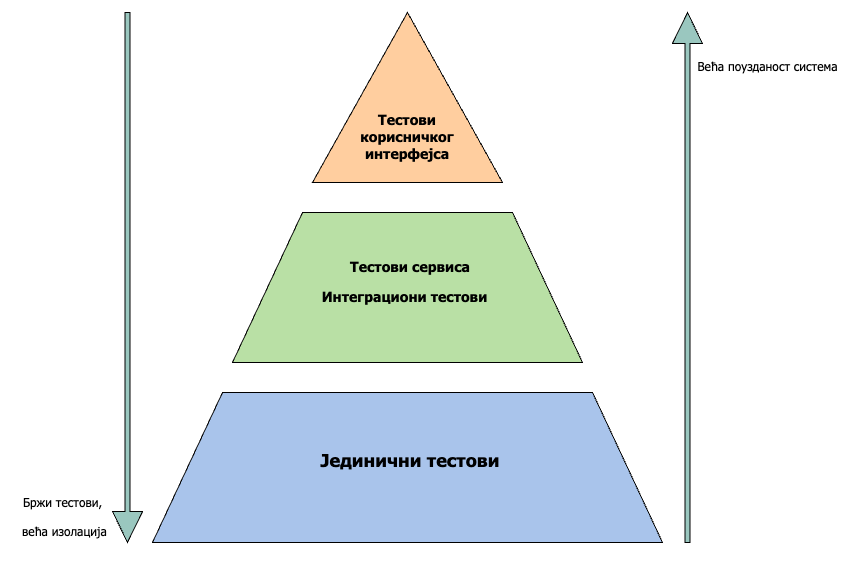
\includegraphics[width=1\textwidth]{matfmaster/img/piramida.png}
  \caption{Модел \textit{пирамиде тестирања}}
  \label{fig:piramida}
\end{figure}

Како су јединични тестови најмањег опсега, логично су и најбржи за извршавање, па је препорука максимално тестирати јединице кода. Аутоматско тестирање интеграција делова система представља начин да поузданост система као целине буде већа, док је цена извршавања и даље мала. Самим тим, тежи се да број ових тестова буде што већи. Тестови корисничког интерфејса представљају скупе операције јер захтевају рад целокупног система, па је приликом одлучивања шта аутоматизовати важно одредити приоритете.

\subsection{Oпсег тестова у контексту микросервисне архитектуре}

Имплементација микросервисне апликације представља компликован процес у ком на различитим деловима апликација често раде другачији тимови. Да би целокупна апликација била поуздана, потребно је тестирати све њене делове у изолацији, као и интеграције тих делова. Коначно, потребно је тестирати апликацију на начин како је корисник користи, односно целокупан систем истовремено.

Микросервисна архитектура, због своје грануларности, омогућава аутоматско тестирање различитих делова апликације у потпуној изолацији, што при коришћењу монолитне архитектуре није могуће. Ово омогућава бржи развој апликације, већу поузданост али и могућност да се модел пирамиде у потпуности примени на систем. 

\section{Тестирање јединица кода}

Јединично тестирање представља проверу исправности појединачних логичких целина у изолацији. Циљ тестова је верификовати да се свака јединица кода понаша у складу са дефинисаним захтевима. Од свих врста тестова, ови тестови су најбржи и најчешће одстрањују велики број грешака. 

Тестови јединица кода се могу писати одмах након, али и пре имплементације одређене функционалности, уколико се користи методологија развоја вођеног тестовима (енг. \textit{Test Driven Development --- TDD}). Одговорност за имплементацију јединичних тестова најчешће преузимају програмери који су радили на самој функционалности, јер је за писање тестова често потребно техничко, али и доменско знање. Познавање граница изоловане функционалности омогућава тестирање  јединице за различите улазне параметре.

Како би се тестови јединица кода исправно аутоматизовали, потребно је комплетно одстранити зависност сваке јединице од остатка система приликом тестирања. Реални подаци од којих зависи функционалност јединице, замењују се ,,лажним” подацима (енг.\textit{ mock data}) који су претходно припремљени. Коришћење овог система има више предности. Одстрањивањем зависности омогућава се тестирање комплексних компоненти апликације које зависе од много улазних параметара, али се и омогућава независно развијање функционалности. Уколико је формат улазних зависности унапред познат, јединица система може несметано имплементирати нове фунцкионалности користећи предефинисане податке.

Јединични тестови су неизоставан део непрекидне интеграције софтвера (енг. \textit{continuous integration}) на основу које се након сваке нове измене покреће скуп аутоматских тестова. Пролазећи кроз итерације испоруке софтвера, јединичним тестовима се осигурава да ни једна нова измена није условила пад неке од постојећих јединица система.

\section{Тестирање интеграција и сервиса}

Поузданост да логичке целине исправно раде у изолацији доприноси укупној поузданости система, али не гарантује да ће интеграција тих целина исправно функционисати. Тестови интеграције проверавају комуникацију између више јединица кода са циљем да пронађу грешке у интерфејсима интегрисаних компоненти.

Аутоматизација интеграционих тестова омогућава брзу проверу комуникације између измењених компоненти у процесу развоја софтвера. Како ова врста тестова покрива веће логичке целине, извршавање тестова је спорије у односу на јединичне тестове, па је и број тестова мањи. 

При коришћењу микросервисне архитектуре, више јединица кода интегрише се у један сервис. Ова интеграција тестира се тестовима сервиса, где је циљ проверити исправност јавног интерфејса који сервис пружа. 

Као што је претходно наведено, микросервисна архитектура подразумева велику грануларност система и самим тим захтева јасан начин комуникације између свих делова система. Како се комуникација одвија између више сервиса, повећава се значај интеграционих тестова. Тестови појединачних сервиса, као и тестови интеграција између различитих сервиса, представљају додатни ниво поузданости који монолитна архитектура не обезбеђује. Пронађена грешка тачно указује која интеграција тј. који интерфејс унутар система не даје очекиване резултате, што значајно олакшава процес елиминације грешке.


\section{Системско тестирање}

Тестови с краја на крај (енг.\textit{ end to end --- e2e}) или тестови корисничког интерфејса, представљају најкомплекснију врсту тестова јер посматрају систем као униформну целину. Пре самог тестирања с краја на крај потребно је тестирати јединице кода, као и интеграције тих јединица. Упркос великој поузданости у квалитет софтвера коју пружају интеграциони и јединични тестови, коришћењем свих делова система истовремено могу се пронаћи проблеми који другачије нису могли бити уочени.

Посматрањем система из угла крајњег корисника добија се реална слика о томе како се систем као целина понаша. Тестови с краја на крај се често извршавају мануелно јер захтевају корисничко развојно окружење и низ комплексних акција које описују случај употребе система. Међутим, алатима који симулирају корисничко понашање могуће је аутоматизовати процес тестирања с краја на крај. Услед комплексности ових тестова, време извшавања је знатно веће од осталих типова тестова па их због тога није практично имати превише. Приликом писања тестова треба осигурати да су изабрани случајеви употребе репрезентативни, односно да осликавају реалну употребу апликације. Слично као и код јединичних тестова, дефинисање случајева употребе који ће се аутоматизовати може се одвијати после, али и пре имплементације функционалности.

Системски тестови имају значајну улогу у методологији агилног развоја софтвера. Покретањем аутоматских системских тестова пре сваке испоруке обезбеђује се сигурност у то да сви покривени случајеви употребе и даље раде. Уколико то није случај, најчешће се генерише извештај који садржи слику или скуп корака који описује како је до грешке дошло.

Како се систем пројектован коришћењем микросервисне архитектуре састоји од много делова који се често не развијају истовремено, системски тестови представљају врло важан корак у развоју апликације. Како би системски тест био исправно извршен, велики број независних делова мора синхроно да функционише. У пракси се дешава да тест падне због разлога који нису нужно везани за функционалност која је тестирана, нпр. због привременог кашњења одговора сервиса.  Тестови који некад пријављују грешку, а некад не, без детерминистичког правила, називају се нестабилни тестови (енг. \textit{flaky tests}). Приликом паралелног извршавања већег броја сличних тестова често долази до нестабилности тестова, услед проблема који се јављају приликом коришћења дељених ресурса.

Нестабилни тестови представљају велики проблем и циљ их је у што већој мери елиминисати. Информација да нестабилан тест пријављује грешку у систему, не доприноси поузданости, јер су разлози због којег тест пада невезани за тестирану функционалност. Уколико се у скупу тестова који се извршавају налази много нестабилних тестова, губи се поверење у валидност резултата тестова. Овај феномен назива се нормализација одступања.



\subsection{Технике тестирања корисничког интерфејса}

Како би се симулирало корисничко понашање при извршавању тестова користе се алати попут развојних оквира \textit{Playwright} \cite{playwright} и \textit{Selenium} \cite{playwrightVsSelenium}. Могуће је аутоматизовати тестове с краја на крај у различитим системима али у склопу овог рада фокус ће бити на веб апликацијама. 

Покретање претраживача у ком се извшавају тестови регулише коришћени развојни оквир, о чему ће бити више речи у поглављу \ref{chp:tehnologije}. Развојни оквир пружа функције за дохватање елемената са странице помоћу кориснички дефинисаних селектора. Селектори представљају шаблоне помоћу којих се одређени елемент може лоцирати на страници апликације, односно унутар \textit{DOM} стабла које претраживач приказује. Специфични развојни оквири подржавају различите типове селектора. Неки од њих су:

\begin{itemize}
\item \textit{CSS} селектори --- лоцирају елементе странице на основу скупа правила која се користе за стилизовање \textit{HTML} eлеменатa,
\item \textit{xpath} селектори --- лоцирају елементе странице на основу путање која дефинише пут кроз \textit{XML} односно \textit{HTML} страну,
\item текстуални селектори --- лоцирају елемент на основу текста који се налази у склопу елемента.
\end{itemize}

Након што је елемент на страници пронађен, случај употребе апликације извршава се помоћу функција које дефинише изабрани алат. Коришћењем библиотека за верификацију проверава се да ли је случај употребе испунио предефинсане захтеве.

Многи случајеви употребе имају преклапајуће скупове корака. Како би се елиминисала редундатност при писању системских тестова, при пројектовању оквира за тестирање користи се модел странице као објекта.

\subsubsection{Mодел странице као објекта}

Модел странице као објекта користи посулате објектно-оријентисаних методологија, конкретно, особине интерфејса и енкапсулације како би раздвојио шта се тестира од начина тестирања са циљем смањења комплексности. 
За сваку страницу апликације или неки смислен функционалан део, прави се класа која представља интерфејс за управљање том страницом. Класа садржи дефиниције селектора који се налазе на датој страници, као и методе помоћу којих се манипулише самом страницом. На овај начин се све информације о страници апликације налазе на једном месту, па су измене при ажурирању тестова минималне. 

Тестови користе дефинисане класе као интерфејсе за извршавање корисничких акција и јасно осликавају случај употребе. Детаљи имплементације сваког корака случаја употребе су сакривени, па је структура теста концизна и јасна. Графички приказ примера имплементације овог архитектуралног модела може се видети на слици \ref{fig:pom}. Пример представља начин моделовања сваке од три странице апликације као и како се те странице користе унутар тестова. Као што је приказано, тестови често користе више различитих интерфејса, јер случај употребе који тестирају обухвата више страница апликације.

\begin{figure}[!ht]
  \centering
  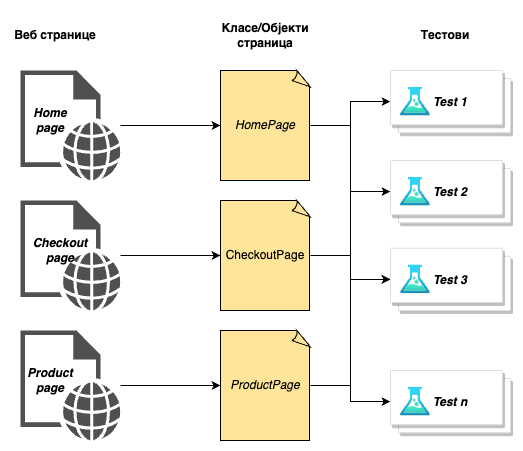
\includegraphics[width=0.8\textwidth]{matfmaster/img/pom.png}
  \caption{Модел странице као објекта}
  \label{fig:pom}
\end{figure}


% ------------------------------------------------------------------------------
\chapter{Имплементација и тестирање апликације \textit{Gelos}}
\label{chp:aplikacija}
% ------------------------------------------------------------------------------
Практични део рада представља имплементацију микросервисне апликације, као и система за тестирање те апликације. Циљ апликације је претраживање и помоћ при избору филма односно књиге за читање. Посебна пажња при изради апликације посвећена је системима за тестирање апликације како на јединичном, тако и на интеграционом и системском нивоу. Архитектурално решење за сваки део овог система је обрађено у склопу овог поглавља. Изворни к\^{o}д апликације и система за тестирање може се видети на \textit{GitHub} страници пројекта \cite{projekat}.

\section{Кратак преглед коришћених технологија}
\label{chp:tehnologije}

За израду микросервиса коришћен је развојни оквир \textit{Express.js} \cite{express} писан за извршно окружење \textit{Node.js} \cite{nodejs}. За складиштење података коришћен је систем за управљање базом података \textit{SQLite} \cite{sqlite} у комбинацији са алатом за објектно-релационо мапирање \textit{Sequelize} \cite{sequelize}. 

За израду клијентске апликације коришћенa jе библиотека \textit{React} \cite{react}. За стилизовање корисничког интерфејса коришћен развојни оквир \textit{Tailwind} \cite{tailwind}. 

За израду оквира за интеграционо и функционално тестирање система коришћен је развојни оквир \textit{Playwright} \cite{playwright} док је за генерисање лажних података за тестирање коришћена библиотека \textit{MSW} (енг. \textit{Mock Service Worker}) \cite{msw}. У склопу израде компонентних и јединичних тестова коришћена је библиотека \textit{React Testing Library} \cite{rtl} у комбинацији са развојним оквиром \textit{Jest} \cite{jest}.

\subsection{Окружење \textit{Node.js}}

\textit{Node.js} представља извршно окружење који омогућава извршавање \textit{JavaScript} кода ван оквира претраживача односно на самом серверу. Могућност да се и клијентска и серверска страна апликације пишу истим програмским језиком и самим тим убрза процес развоја апликације, допринела је великој популарности језика.
Ипак, главну особину овог развојног оквира представља могућност да извршава неблокирајући, асинхрон к\^{o}д и тако елиминише потребу за чекањем  \cite{w3nodejs}.

У склопу овог пројекта коришћен је и \textit{npm} (енг. \textit{node package manager}) који омогућава једноставну контролу инсталација и верзија коришћених библиотека \cite{npm}. Како се пројекат састоји из више независних целина коришћена је "\textit{monorepo}" стратегија за контролу верзија. Ова стратегија омогућава развијање више независних пројеката унутар истог репозиторијума, као и независно покретање сваког од делова система \cite{monorepo}.

\subsection{Развојни оквир \textit{Express.js}}

Инспирисан развојним оквиром \textit{Sinatra} \cite{sinatra}, \textit{Express.js} се одликује својом једноставношћу, уз могућност да кроз различите библиотеке испуни специфичне захтеве апликације. \textit{Express.js} пружа минималан скуп функционалности које омогућавају једноставну обраду \textit{HTTP} захтева, рутирање и интеграцију са системом за управљање базама података \cite{express}. 

Како \textit{Express.js} представља веома ниску апстракцију \textit{HTTP} протокола, има врло добре перформансе, па је због те особине и своје једноставности постао стандардан алат за креирање веб сервера и програмских интерфејса апликације унутар \textit{Node.js }окружења \cite{mdnexpress}.

\subsection{Систем за управљање базама података \textit{SQLite} и библиотека \textit{Sequelize}}

\textit{SQLite} је систем за управљање базама података написан у програмском језику \textit{C}. Дизајниран је тако да буде стабилан, брз и компатибилан са различитим платформама.  Насупрот другим \textit{SQL} системима за управљање базама података, нема засебан серверски процес већ комплетну базу података чува унутар једне датотеке \cite{sqlite,sqlitetutorial}

Објектно-релационо мапирање представља технику која омогућава да се подацима из базе података приступа користећи парадигму објектно оријентисаног програмирања. Ова техника омогућава да се подацима приступа кроз објекте односно методе тих објеката па се компликовани \textit{SQL} упити апстрахују у интуитивне позиве функција. У потпуности се елиминише потреба за употребом \textit{SQL} језика па то додатно убрзава процес развоја софтвера \cite{orm}. \textit{Sequelize} је библиотека за објектно релационо мапирање која је заснована на технологији \textit{ Node.js} и подржава велики број система за управљање базама података попут \textit{Postgres, MySQL, MariaDB, Microsft SQL Server} и \textit{SQLite} \cite{sequelize}.

\subsection{Библиотека \textit{React}}
\label{section:react}
Библиотека \textit{React} представља једну од најпопуларнијих \textit{JavaScript} библиотека за израду корисничког интерфејса.  Почива на идеји да се свака апликација састоји од скупа компоненти које представљају енкапсулиране целине. Свака компонента представља вид шаблона па се може употребити више пута са различитим параметрима што смањује редундантност написаног кода. Како су компоненте јединичне целине оне у себи садрже и приказ саме компоненте у виду \textit{HTML} елемената и \textit{CSS} правила, као и начин на који се те компоненте мењају, у виду \textit{JavaScript} кода \cite{react}.

\textit{React} прави виртуелно \textit{DOM} (енг. \textit{Document Object Model}) стабло које ажурира право \textit{DOM} стабло само за компоненте које су промењене при некој акцији на корисничком интерфејсу. Ово омогућава да се промене дешавају брже и без ажурирања целе веб странице што омогућава креирање такозваних једностраничних апликација \cite{react}. 

Сама библиотека имплементира само основне функционалности потребне за креирање корисничког интерфејса док се за функционалности попут рутирања морају инсталирати додатне библиотеке. Једна од таквих је библиотека \textit{React router} која је коришћена у склопу овог пројекта \cite{reactRouter}.

\subsection{Развојни оквир \textit{Tailwind} }

Стилизовање модерних веб страница које се приказују другачије у односу на величину екрана уређаја представља велики изазов у процесу развоја веб апликације. Појава \textit{CSS} развојних оквира који садрже већ стилизоване шаблоне омогућила је једноставно имплементирање модерног корисничког интерфејса. Коришћењем већ постојећих шаблона губи се могућност за прављењем јединственог корисничког интерфејса па се и поред развојних оквира као што је \textit{Bootstrap} користе и стандардна \textit{CSS} правила \cite{bootstrap}.

\textit{Tailwind} представља \textit{CSS} развојни оквир који решава проблем на мање рестриктиван начин, задржава брзину и једноставност развоја коју пружају горе поменути развојни оквири, а дозвољава флексибилност коју пружа коришћење \textit{CSS} правила. То се постиже коришћењем предефинисаних класа које у себи садрже велики број функционалности које омогућавају кориснику да лако имплементира комплексне промене на корисничком интерфејсу \cite{tailwind}.


\subsection{Развојни оквир \textit{Playwright}}

\textit{Playwright} је развојни оквир направљен за аутоматизацију системских тестова од стране \textit{Microsoft} тима. Оквир подржава више програмских језика као што су \textit{Јava}, \textit{Python}, \textit{C\#}  и \textit{JavaScript} \cite{playwright}.

Сваки претраживач садржи погонски део који је одговоран за трансформисање \textit{HTML} текста у веб страницу која се приказује на самом уређају. \textit{Playwright} користи протокол \textit{DevTools} који омогућава директну комуникацију са погонским делом претраживача у циљу извршавања тестова у претраживачу \cite{playwrightTutorial}. Ова особина чини оквир знатно бржим и стабилнијим од конкуретних технологија које користе протокол \textit{WebDriver}. \cite{playwrightVsSelenium,speedTest}. Оквир подржава извршавање на претраживачима као што су \textit{Chromium,  Firefox} и \textit{Webkit} \cite{playwright, chromium,webKit}.

Једна од главних особина оквира је аутоматско чекање. Пре сваке акције над елементом на веб страници, проверава се да ли је елемент видљив и активан па се тек онда наставља са извршавањем теста. Ово елиминише потребу за имплицитним чекањима у аутоматским тестовима. Имплицитна чекања, односно заустављање теста на предефинисан број секунди како би се одређен елемент учитао, представљају чест узрок нестабилних тестова. Аутоматско чекање такође смањује потребу за експлицитним чекањима, која заустављају тест док одређен услов није испуњен, јер се већина стандардно коришћених услова аутоматски проверава пред интеракцију са елементом. Смањен број експлицитних чекања у тесту доприноси томе да тест буде концизан и јасан.

Конкурентно извршавање тестова је подржано и једноставно се имплементира услед асинхроне природе \textit{Node.js} оквира. Оквир не подржава тестирање на реалним мобилним уређајима али подржава емулацију претраживача за мобилне телефоне.

Уз алате за тестирање корисничког интерфејса, \textit{Playwright} такође пружа алате за визуелно тестирање, компонентно тестирање, и тестирање програмских интерфејса апликације \cite{playwright}. Неки од тих алата биће приказани у даљем тексту.

\subsection{Библиотека за тестирање \textit{React} апликација и  библиотека \textit{Jest}}

Тестирање појединачних јединица и компоненти система који користи библиотеку \textit{React} може се постићи коришћењем библиотеке за тестирање \textit{React} апликација (енг.\textit{ React testing library}) \cite{rtl}. Библиотека омогућава тестирање појединачних чворова \textit{DOM} стабла из угла корисника. Свака \textit{React} компонента се претвара у \textit{DOM} чвор и помоћу \textit{JavaScript} библиотеке за тестирање --- \textit{Jest}, проверавају се очекиване вредности унутар чвора. Ова библиотека пружа сигурност да се подаци приказују на очекиван начин без обзира на друге делове система, као и да различите јединице функционишу унутар компоненти којима припадају \cite{rtl,jest}.


\subsection{Библиотека \textit{MSW}}

Како би тестови били поуздани и подаци који се користе унутар тестова морају бити поуздани. Такође потребно је тестирати клијентски део апликације независно од серверског дела. 

\textit{MSW} (енг. \textit{Mock Service Worker}) представља библиотеку која омогућава да се \textit{API} позиви који су упућени ка серверској страни апликације пресретну и уместо правих, клијентској апликацији врате предефинисани ,,лажни” одговори. Ово омогућава како тестирање клијентског дела апликације у изолацији, тако и могућност независног развоја клијентског и серверског дела апликације \cite{msw}. Да би одговарајући \textit{API} позиви били пресретнути потребно је дефинисати тачке јавног интерфејса и предефинисане податке који се шаљу клијентској страни апликације.

% ОВДЕ МОЖЕ СЛИКА MSW


\section{Архитектура и дизајн апликације}

Развијена апликација подељена је у две целине, на серверски и клијентски део. Серверски део апликације организован је у међусобно незавнисне микросервисе. Сваки микросервис има јасно дефинисан јавни интерфејс помоћу ког клијентска страна апликације приступа ресурсима и функционалностима које микросервис пружа. Подаци које микросервиси користе организовани су тако да сваки микросервис има своју базу података. Комуникација између микросервиса и клијентског дела апликације извршава се коришћењем \textit{HTTP} протокола. У наставку ове секције биће детаљније приказани имплементациони детаљи као и архитектурална решења за сваки од делова апликације.


\subsection{Микросервиси}

Серверски део апликације састоји се од два независна микросервиса \textit{Movies} и \textit{Books}. Архитектура коришћена при имплементацији оба микросервиса је \textit{Модел-Поглед-Контролер} па је структура пројекта подељена у одговарајуће целине:
\begin{enumerate}
\item Покретање и јавни интерфејс микросервиса (у кореном директоријуму):
\begin{itemize}
\item Датотека \textit{index.js} --- покреће претходно дефинисан сервер на одговарајућем порту.
\item Датотека \textit{server.js} --- дефинише јавни интерфејс микросервиса.
\end{itemize}
\item Рутери (у директоријуму \textit{routers}) --- повезују добијене \textit{HTTP} захтеве са компонентама које су одговорне за обраду тих захтева.
\item Контролери (у директоријуму \textit{controllers}) --- имплементирају бизнис логику микросервиса тако што обрађују захтеве и делегирају операције доменским моделима.
\item Описи и методе за иницијализацију модела (у директоријуму \textit{models}) ---  дефинишу поља модела и имплементирају методе које учитавају и парсирају податке из базе података.
\item Конфигурација  система за управљање базом података (у директоријуму \textit{services}) --- конфигурише објектно-релационо мапирање и путању до фајла у ком се налази база података.
\end{enumerate}


\subsubsection{Сервис \textit{Movies}}

Сервис \textit{Movies}, односно сервис филмова, је сервис задужен за управљање подацима о филмовима и оценама за те филмове. Доменски модел овог сервиса налази се на слици \ref{fig:moviesShema}. Ентитет \textit{Title} садржи податке о филму као што су име, година снимања, број минута и жанр филма, док ентитет \textit{Rating} садржи информације о просечној оцени као и о броју корисника који су дали оцену за филм на сајту \textit{IMDB}.

\begin{figure}[!ht]
  \centering
  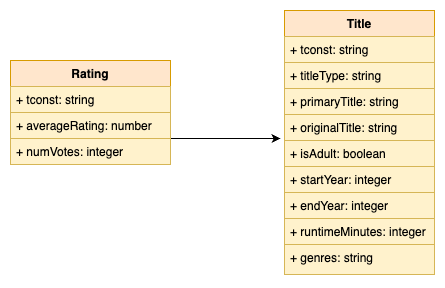
\includegraphics[width=0.75\textwidth]{matfmaster/img/moviesShema.png}
  \caption{Доменски модел сервиса \textit{Movies}}
  \label{fig:moviesShema}
\end{figure}
Сервис пружа јавни интерфејс помоћу ког је могуће добити информације о свим филмовима, о специфичном филму на основу његовог идентификатора као и добити листу филмова на основу упита. Детаљнији опис интерфејса приказан је у табели \ref{tbl:moviesAPI}.
\newpage
\begin{table}
\caption{Опис јавног интерфејса сервиса  \textit{Movies} }
\label{tbl:moviesAPI}
\begin{center}
\begin{tabular}{ |  p{0.3\linewidth} | p{0.3\linewidth}|  p{0.4\linewidth} | }
 
 \hline
  \textit{Опис} & \textit{Параметри} & \textit{Одговор при успешној обради} \\
  \hline
  \multicolumn{3}{|c|}{\textbf{GET api/v1/version}} \\
  \hline
  Дохватање актуелне верзије интерфејса
  & 
  
  & 
 \textit{version} --- тренутна верзија интерфејса \\
  \hline
 \multicolumn{3}{|c|}{\textbf{GET api/v1/movies}} \\
  \hline
  Дохватање информација о свим доступним филмовима
  & 
  \textit{pagе} --- број странице резултата (oпционо) \newline 
  \textit{size} --- број филмова на страници (опционо)
  & 
  \textit{data} --- објекат који садржи листу филмова са оценама \newline  
  \textit{meta} --- објекат који саджи мета податке о листи \\
  \hline
   \multicolumn{3}{|c|}{\textbf{GET api/v1/movies/:id}} \\
  \hline
  Дохватање информација о специфичном филму 
  & 
  \textit{id} --- идентификатор филма (обавезно)
  & 
  \textit{data} --- објекат који садржи информације о специфичном филму\\
  \hline
   \multicolumn{3}{|c|}{\textbf{GET api/v1/movies/search}} \\
  \hline
  Претрага филмова на основу имена филма
  & 
  \textit{pagе} --- број странице резултата (oпционо) \newline 
  \textit{size} --- број филмова на страници (опционо) \newline 
  \textit{query} --- кључна реч за претрагу (обавезно)
  & 
  \textit{data} --- објекат који садржи листу филмова \newline  
  \textit{meta} --- објекат који саджи мета податке о листи \\
   \hline
     \multicolumn{3}{|c|}{\textbf{GET api/v1/ratings}} \\
  \hline
 Дохватање свих оцена филмова
  & 
  \textit{pagе} --- број странице резултата (oпционо) \newline 
  \textit{size} --- број филмова на страници (опционо)
  & 
  \textit{data} --- објекат који садржи листу o оцена филмова са њиховим насловом \newline 
  \textit{meta} --- објекат који саджи мета податке о листи \\ 
  \hline
\end{tabular}
\end{center}
\end{table}

\newpage

\subsubsection{Сервис \textit{Books}}

Сервис \textit{Books}, односно сервис књига, је сервис задужен за управљање подацима о популарним књигама. Сервис омогућава претрагу популарних наслова, као и добијање информација о аутору, оцени наслова и других информација о књигама. Доменски модел овог сервиса налази се на слици \ref{fig:booksShema}. 
Сервис пружа програмски дефинисан интерфејс који омогућава излиставање целокупне листе књига које се налазе у бази података, као и претрагу по насловима.
\newpage

Сервис књига има врло сличан јавни интерфејс као и сервис филмова, али због разлика у доменима и количини података са којима располажу, овај сервис у склопу исте табеле садржи информације о књигама и инфомације о оценама тих књига. Детаљан опис функционалности које микросервис пружа може се видети у табели \ref{tbl:booksAPI}.


\begin{table}
\caption{Опис јавног интерфејса сервиса \textit{Books}}
\label{tbl:booksAPI}
\begin{tabular}{ |  p{0.3\linewidth} | p{0.3\linewidth}|  p{0.4\linewidth} | }
\hline
\textit{Oпис} & \textit{Параметри} & \textit{Одговор при успешној обради} \\
\hline
\multicolumn{3}{|c|}{\textbf{GET api/v1/version}} \\
\hline
Дохватање актуелне верзије интерфејса & & 
\textit{version} --- тренутна верзија интерфејса \\
\hline
\multicolumn{3}{|c|}{\textbf{GET api/v1/books/}} \\
\hline
Дохватање информација о свим доступним књигама & 
\textit{pagе} --- број странице резултата (oпционо) \newline 
\textit{size} --- број књига на страници (опционо)
& 
\textit{data} --- објекат који садржи листу књига \newline
\textit{meta} --- објекат који саджи мета податке о листи \\
\hline
\multicolumn{3}{|c|}{\textbf{GET api/v1/books/search}} \\
\hline
Претрага књига на основу наслова књиге &
\textit{pagе} --- број странице резултата (oпционо) \newline 
\textit{size} --- број књига на страници (опционо) \newline 
\textit{query} --- кључна реч за претрагу (обавезно) 
  & 
\textit{data} --- објекат који садржи листу књига \newline
\textit{meta} --- објекат који саджи мета податке о листи \\
\hline
\end{tabular}
\end{table}


\begin{figure}[!ht]
  \centering
  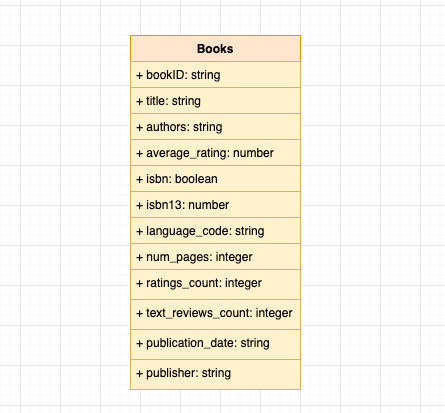
\includegraphics[width=0.5\textwidth]{matfmaster/img/booksShema.png}
  \caption{Доменски модел сервиса \textit{Books}}
  \label{fig:booksShema}
\end{figure}
\newpage

\newpage


\subsection{Kлијентска апликација}

У склопу пројекта направљена је клијентска апликација која користи фукционалности које имплементирани микросервиси пружају. За имплементацију коришћена је библиотека \textit{React} као и помоћнa библиотекa \textit{React router} \cite{reactRouter}. Апликација је подељена на компоненте које представљају изоловане целине система и у себи садрже логику и визуелни приказ дела апликације.

Централни део хијерархијске структуре апликације имплементиран је у компоненти \textit{Аpp}. Она сваку компоненту приказује унутар компоненте \textit{Layout} која дефинише распоред компоненти на страници, и изнад и испод сваке странице приказује компоненту \textit{Header} и \textit{Footer} респективно. \textit{Header} имплементира заглавље које садржи мени за навигацију, док \textit{Footer} представља подножје странице. Коришћењем библиотеке \textit{React router}, компонента \textit{App} приказује одговарајућу страницу у зависности од \textit{URL} путање. Уколико је путања неисправна биће приказана компонента \textit{Page404} која корисника обавештава о неисправно унешеној путањи.  

Странице интегришу више компоненти и имплементирају комуникацију са серверским делом апликације. Страница \textit{Homepage} представља полазну тачку клијентске апликације и приказује више презентационих картица које користе податке дефинисане у \textit{contents} директоријуму. Навигацијом кроз презентационe картицe или кроз горњи мени за навигацију корисник се преусмерава на неку од страница. 

Страница \textit{MoviesPage} омогућава кориснику презентацију као и претрагу оцењених филмова. Компонента  \textit{MoviesPage} користи јавни интерфејс \textit{Movies} сервиса и у складу са корисничким уносом података приказује листу филмова односно компоненти \textit{Movie}.  У склопу ове странице имплементирано је и приказивање вишестраничних резултата упита кроз компоненту \textit{Pagination}. Аналогно, страница \textit{BooksPage} приказује листу књига и омогућава претрагу књига по њиховом наслову користећи јавни интерфејс \textit{Books} сервиса. Обе компоненте користе компоненту \textit{SearchBar} која регулише унос наслова за претрагу. Празан унос у поље за претрагу кориснику враћа иницијалан скуп података.

Структура директоријума клијентске апликације осликава функционалност сваке од компоненти апликације. Компоненте које представљају странице апликације налазе се у директоријуму \textit{pages} док се компоненте које представљају делове страница налазе у директоријуму \textit{components}. Искључиво презентационе компоненте попут \textit{Loading} или \textit{Icons} компоненти налазе се у директоријуму \textit{ui}. Поред конфигурационих датотека у склопу апликације се налазе и систем за тестирање апликације као и систем за пресретање \textit{API} позива о којима ће бити речи у наредном поглављу. Графички приказ клијентске апликације приказан је на слици \ref{fig:client}.

\begin{figure}[!ht]
  \centering
  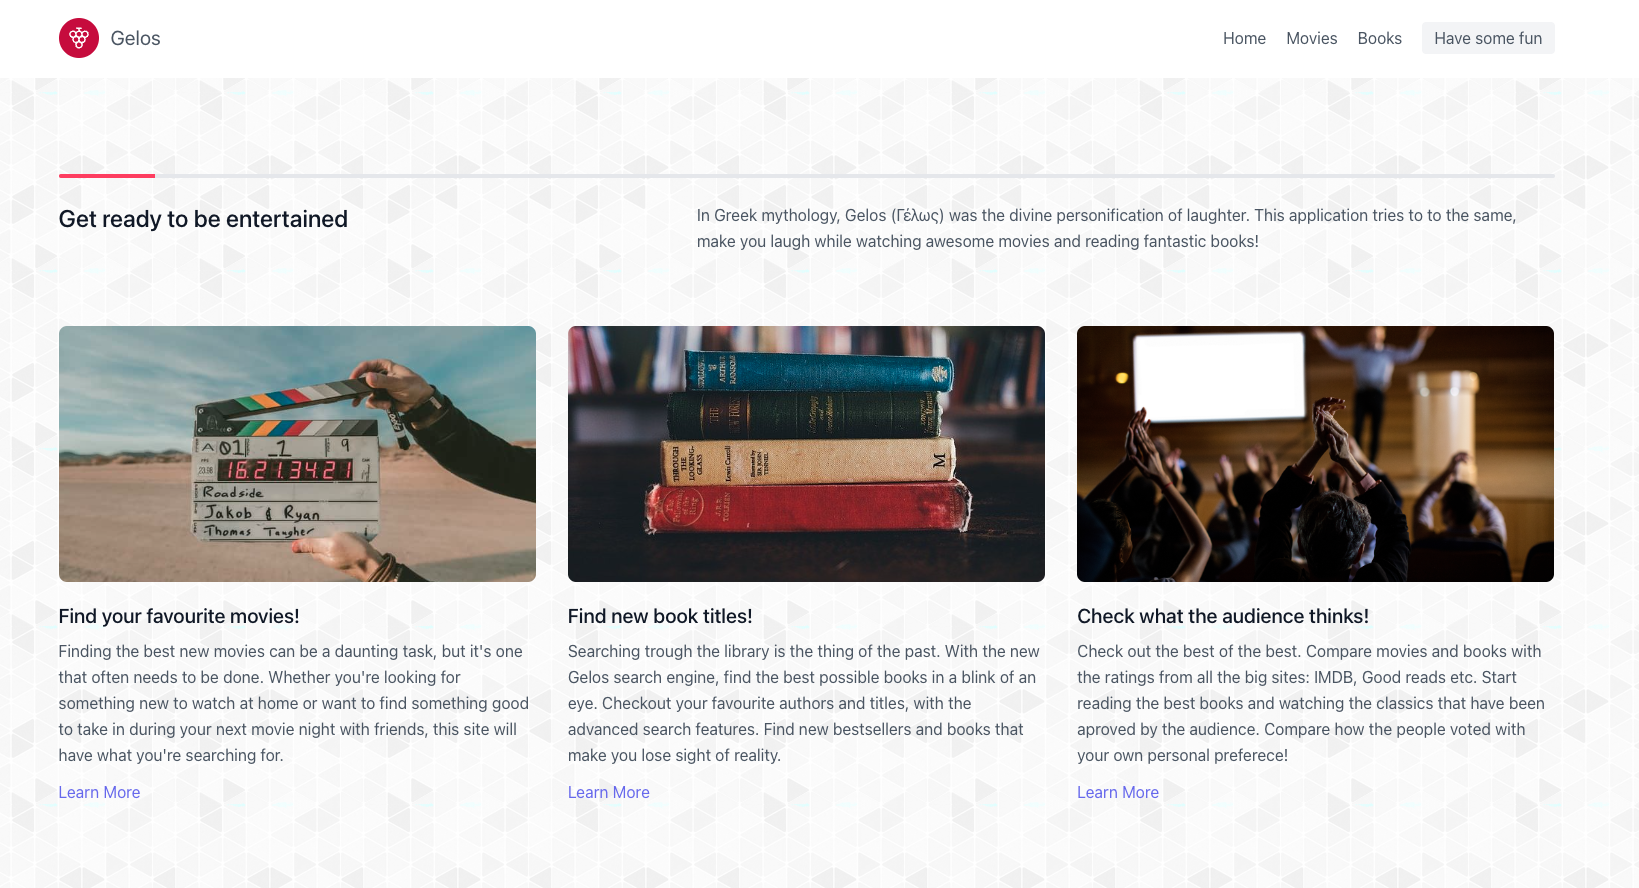
\includegraphics[width=\textwidth]{matfmaster/img/client.png}
  \caption{Клијентска апликација \textit{Gelos}}
  \label{fig:client}
\end{figure}
\newpage
\section{Аутоматско тестирање апликације}

Систем за тестирање апликације имплементиран је на више нивоа, па су у слопу пројекта дефинисани јединични, интеграциони и системски тестови. Свака врста тестова доприноси поузданости целокупне апликације и омогућава лако налажење проблема при развоју нових или изменама постојећих функционалности.

Јединичним тестовима проверена је исправност сваке функционалне компоненте клијентске апликације у изолацији, уз помоћ система за пресретање \textit{API} позива. Странице апликације као и мање компоненте које чине те странице покривене су тестовима па је укупно имплементирано ??? јединичних тестова.

Интеграција клијентске апликације и микросервиса проверава се тестовима дефинисаним у директоријуму \textit{integration}. Тестови су груписани у два скупа у зависности од интеграције коју тестирају, а свака група се састоји од осам различитих тестова, па је укупно имплементирано шеснаест тестова.

Како је потребно тестирати апликацију на начин како је корисник користи, имплементирани су тестови који тестирају целокупан систем. Тестови су дефинисани у директоријуму \textit{e2e} и покривају најчешће случајеве употребе. Имплементирано је двадесет два теста који се извршавају на три различита претраживача.  Тестови су подељени у пет група у зависности од функционалности коју проверавају.

У наставку ове секције биће детаљно приказани имплементациони детаљи аутоматских тестова на различитим нивоима, док ће на крају поглавља бити речи о временским оквирима извршавања тестова.

\subsection{Јединично тестирање апликације}

Како јединично тестирање апликације представља проверу исправности појединачних логичких целина у изолацији потребно је дефинисати те целине и окружење у којем их је могуће тестирати. Свака од \textit{React} компоненти може се посматрати као изолован део клијентске апликације. Тестирање ових компоненти у изолацији могуће је само уз одстрањивање зависности од остатка система. To се постиже коришћењем библиотеке за тестирање \textit{React} апликација и библиотеке \textit{MSW}.

Тестирање сваке компоненте састоји се од генерисања \textit{DOM} стабла за ту компоненту, и провере да ли се компонента приказује и мења у складу са предефинисаним очекивањима. Тестови су ради прегледности названи идентично као и компоненте које тестирају уз наставак \textit{.test}. 

У наставку је представљен  к\^{o}д који тестира компоненту \textit{SearchBar} односно поље за претрагу филмова или књига. Након генерисања \textit{DOM} стабла компоненте (линија 5), проверава се да ли се поље за унос и дугме за претрагу налазе унутар стабла (линије 9 и 10). После уноса текста у поље проверава се да ли је вредност исправно унешена у поље (линија 13). На овај начин се тестира функционалност поља за унос без обзира на резултате претраге или друге компоненте које се користе у комбинацији са \textit{SearchBar} компонетом.

\begin{lstlisting}[caption=Јединично тестирање \textit{SearchBar} компоненте,
label={lst:searchbarTest},
frame=single]
import { fireEvent, render, screen } from "@testing-library/react";
import SearchBar from "../components/SearchBar.jsx";

test("Search bar unit test", async () => {
  render(<SearchBar></SearchBar>);
  let searchField = screen.getByPlaceholderText("Search by title");
  let searchButton = screen.getByRole('button')
  
  expect(searchField).toBeInTheDocument();
  expect(searchButton).toBeInTheDocument();

  fireEvent.change(searchField, { target: { value: "Some random query" } });
  expect(searchField.value).toBe("Some random query");
});
}
\end{lstlisting}

Аналогно за сваку од јединичних компоненти које има смисла тестирати попут компоненти које су одговорне за приказивање појединачне књиге (\textit{Book}) односно филма (\textit{Movie}), покреће се тест који проверава исправно генерисање \textit{DOM} стабла за предефинисане податаке. Покретањем ових тестова смањује се могућност неисправног приказа компоненти како за исправне тако и за неисправне уносе.
 
\subsubsection{,,Лажни” подаци}

Неке од \textit{React} компоненти при покретању користе више мањих компоненти као и податке које пружају микросервиси. Циљ је тестирати овакве компоненте независно од \textit{backend} система.

Приликом покретања јединичних тестова заустављају се \textit{API} позиви упућени ка микросервисима и враћају се ,,лажни” одговори који се користе при проверама унутар самог теста.  Коришћењем овог система, странице \textit{BookPage} и \textit{MoviePage} се тестирају  у изолацији без обзира на то да ли микросервиси исправно функционишу јер користе предефинисан скуп података.

Уколико приликом покретања клијентског дела апликације променљива окружења \textit{MOCK\_DATA} има позитивну вредност, сви позиви ка микросервисима биће пресретнути од стране поменутог система и користиће се подаци дефинисани у датотеци \textit{mockData.json}. У склопу директоријума \textit{mocks} налазе се следеће датотеке:

\begin{itemize}
\item \textit{server.js} --- иницијализује систем за пресретање позива у тестовима,
\item \textit{handlers.js} --- дефинише који ,,лажни” подаци ће се вратити за сваку од дефинисаних путања,
\item \textit{mockData.json} --- скуп ,,лажних” података,
\item \textit{browser.js} --- иницијализује систем за пресретање позива при покретању клијентске апликације.
\end{itemize}


\subsection{Тестирање интеграција апликације}

Интеграција између микросервиса и клијентске апликације одвија се коришћењем \textit{HTTP} протокола. Помоћу библиотеке \textit{Playwright} имплементирани су тестови који шаљу \textit{API} позиве ка јавним интерфејсима микросервиса и проверавају да ли су добијени резултати у складу са очекивањима клијентског дела апликације. У зависности од прослеђених параметара тестирају се различити очекивани резултати.

У наставку је представљен један тест који тестира интеграцију између клијентске апликације и сервиса \textit{Movies}, тако што проверава да ли приликом узимања скупа филмова без прослеђених параметара клијент добија податке у очекиваном формату. Након слања \textit{API} позива сервису (линија 2), проверава се статус самог одговора (линија 3) и очекиване вредности за мета параметре (линија 5). Затим се проверавају типови добијених вредности за сваки од филмова, као и да ли су подаци исправни  (линија 10) , односно у очекиваном опсегу вредности (линије 11 и 12). Овим проверама се значајно повећава сигурност да ће подаци који су добијени од стране микросервиса бити исправно приказани на клијентској страни апликације.

\begin{lstlisting}[caption= Тест интеграције сервиса \textit{Movies} и клијентске апликације, 
language=Javascript,
label={lst:integrationTest},
frame=single]
test("Get movies test - no parameters", async ({ request }) => {
    const response = await request.get(`${baseUrl}/api/v1/movies`);
    expect(response.status()).toBe(200);
    const responseBody = JSON.parse(await response.text());
    verifyMetaValues(responseBody.meta, defaultPage, defaultItemsPerPage);

    let movies = responseBody.data.movies;
    expect(movies.length).toBe(defaultItemsPerPage);
    movies.forEach((movie) => {
      verifyMovieTypes(movie);
      verifyMovieLimits(movie);
      verifyMovieRatingLimits(movie.Rating);
    });
  });
\end{lstlisting}

Тестови су груписани у складу са интеграцијом коју тестирају, па се тестови који проверавају конекцију између клијентске апликације и сервиса \textit{Movies} односно \textit{Books} налазе у датотеци \textit{moviesTests} и \textit{booksTests} респективно. Сваки скуп тестова се може независно покретати, што је корисно у случају да је потребно тестирати утицај промена на само једну интеграцију. Директоријум \textit{helpers} садржи помоћне функције за верификацију типова и вредности података који се тестирају.

Након извршавања тестова интеграције генерише се веб страница са извештајем који приказује колико је тестова успешно или неуспешно извршено. За сваки од тестова могуће је видети на ком је кораку пао, па се јасно може утврдити место у систему у ком се налази грешка. Пример извештаја након извршавања интеграционих тестова може се видети на слици \ref{fig:integrationReport}.

\begin{figure}[!ht]
  \centering
  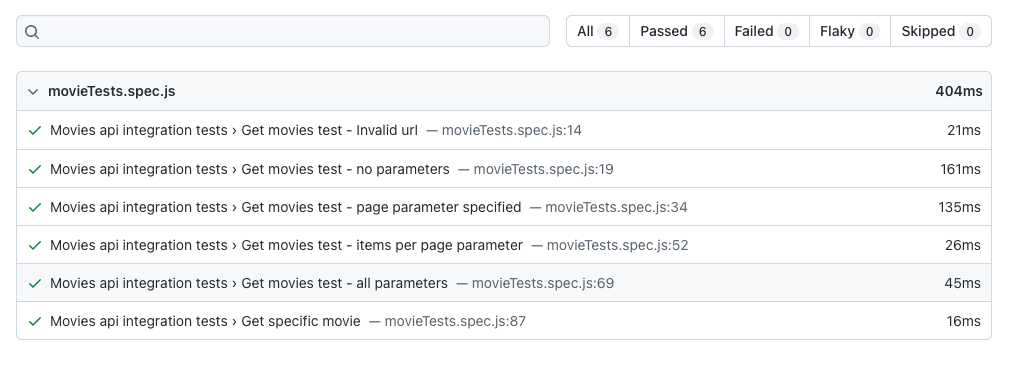
\includegraphics[width=0.75\textwidth]{matfmaster/img/integrationReport.png}
  \caption{Извештај након извршавања интеграционих тестова за сервис \textit{Movies}}
  \label{fig:integrationReport}
\end{figure}
\newpage
\subsection{Тестови система}

Комплексност микросервисне архитектуре лежи у чињеници да се систем састоји од много независних компоненти које треба кохезивно да функционишу. Системско тестирање микросервисне апликације подразумева проверу да ли целокупан систем испуњава претходно дефинисане захтеве.

Развојни оквир \textit{Playwright} омогућава аутоматско покретање претраживача и тестирање апликације из угла корисника. На овај начин могуће је тестирати различите случајеве употребе система на брз и поновљив начин. Случајеви употребе који нису међусобно зависни могу се извршавати паралелно и на тај начин додатно убрзати процес тестирања с краја на крај, које важи за најспорију врсту тестирања.

Архитектурално решење коришћено за имплементацију системских тестова  је модел странице као објекта. Класе које дефинишу елементе и методе на свакој од страница налазе се у директоријуму \textit{pages}. 

Страница \textit{BasePage} представља базну класу за све друге странице и садржи опис елемената који се налазе на свакој страници апликације као и методе које управљају тим елементима.  Свака од страница у конструктору садржи селекторе који описују елементе странице апликације. Странице \textit{BookPage}, \textit{MoviePage} и \textit{HomePage} имплементирају интерфејсе за управљање главним страницама апликације, док су странице \textit{Navbar} и \textit{Footer} одговорне за управљање доњим и горњим менијем апликације респективно.

Тестови се налазе у директоријуму \textit{е2е} и користећи интерфејс који пружају описане странице апликације тестирају функционалности система. Група тестова имплементирана је у једној датотеци. Тестови из исте групе извршавају се секвенцијално док се тестови из различитих група извршавају паралелно. Максималан број паралелних процеса као и друге конфигурационе променљиве дефинисане су у датотеци \textit{playwright.config}. Детаљан приказ архитектуре коришћене за имплементацију налази се на слици \ref{fig:arhitektura}.

\begin{figure}[!ht]
  \centering
  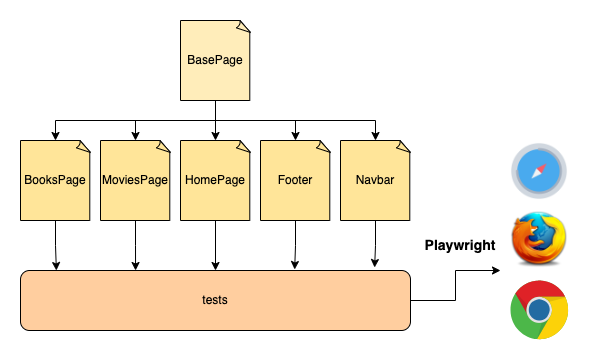
\includegraphics[width=0.75\textwidth]{matfmaster/img/arhitektura.png}
  \caption{Архитектурално решење системских тестова}
  \label{fig:arhitektura}
\end{figure}

У наставку је представљен тест који проверава случај употребе претраге књига где је очекиван резултат претраге цела страница резултата. Коришћењем дефинисаних интерфејса страница проверава се очекиван број резултата на страници (линија 6) као и укупан очекиван број резултата (линија 7).


\begin{lstlisting}[caption=Тест случаја употребе --- претрага књига, 
label={lst:pretragaKnjiga},
frame=single]
 test("Valid search query - full page result", async ({ page }) => {
    const booksPage = new BooksPage(page);
    let numOfMovies = await booksPage.getNumOfBooksOnPage();
    let totalNumOfResults = await booksPage.getTotalNumOfBooks();
    await booksPage.search("Harry");
    await booksPage.verifyNumOfBooksOnPageEquals(numOfMovies);
    await booksPage.verifyTotalNumOfBooksLessThen(totalNumOfResults);
  });
\end{lstlisting}

Системским тестовима покривени су најчешћи случајеви употребе апликације из угла корисника. Тестови су подељени у следеће групе:
\begin{itemize}
\item \textit{footerTests} --- група тестова за проверу функционалности заглавља странице,
\item \textit{navigationTests} --- група тестова за проверу функционалности горњег навигационог менија,
\item \textit{paginationTest} --- група тестова за проверу функционалности страничења на свим страницама које приказују више података,
\item \textit{searchBookTests} --- група тестова за проверу функционалности претраге књига,
\item \textit{searchMovieTests} --- група тестова за проверу функционалности претраге филмова.
\end{itemize}

Након извршавања групе системских тестова генерише се извештај у форми веб странице где је приказан проценат успешности тестова. Приказ извештаја након једног извршавања скупа тестова приказан је на слици \ref{fig:e2e}. Навигацијом кроз извештај могуће је видети који случај употребе и из ког разлога није успешно извршен. Извештај такође садржи и снимак екрана у оном тренутку када је тест неуспешно завршен што се може видети на слици \ref{fig:error}.
 
 
 \begin{figure}[!ht]
  \centering
  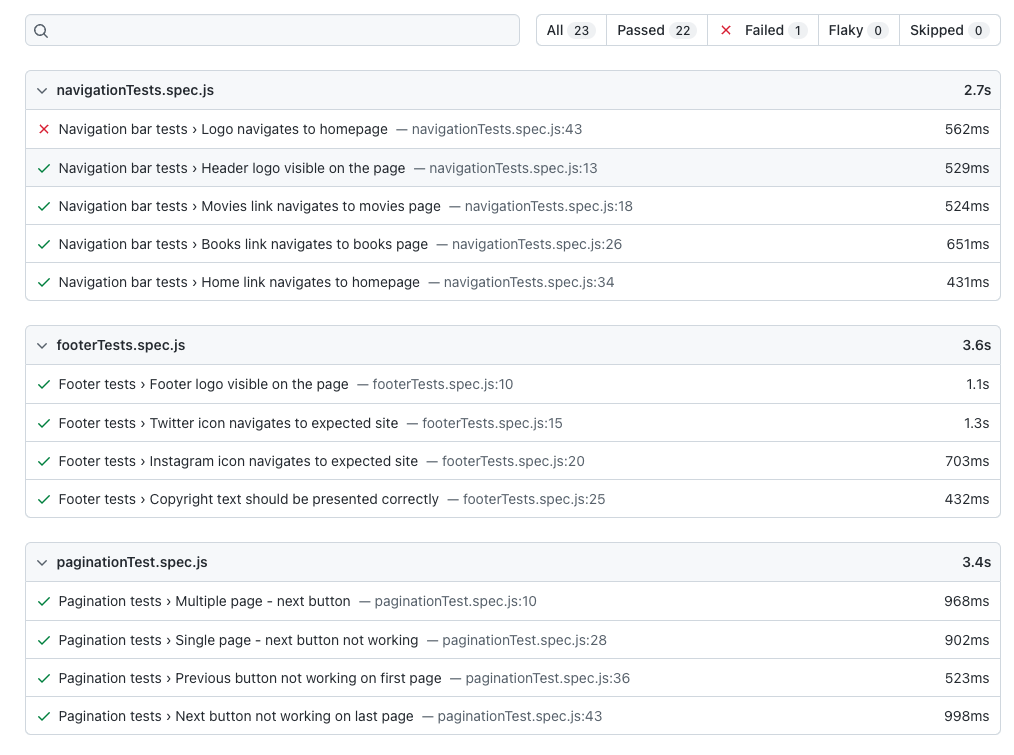
\includegraphics[width=0.75\textwidth]{matfmaster/img/e2e.png}
  \caption{Пример извештаја приликом извршавања скупа системских тестова}
  \label{fig:e2e}
\end{figure}



 \begin{figure}[!ht]
  \centering
  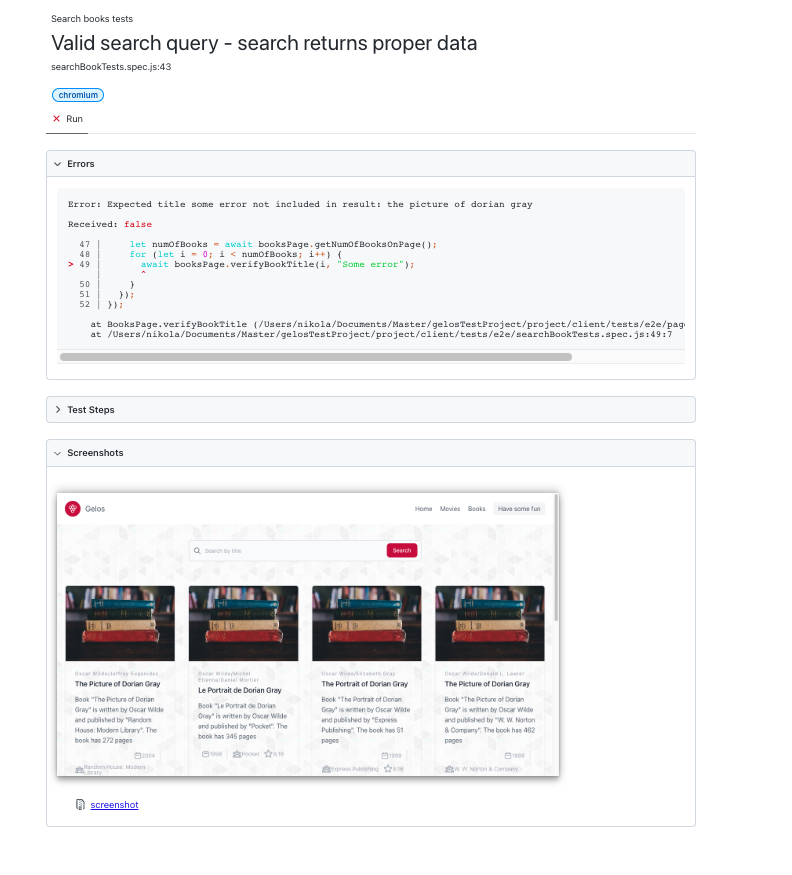
\includegraphics[width=0.75\textwidth]{matfmaster/img/error.png}
  \caption{Пример извештаја за неуспешно завршен тест}
  \label{fig:error}
\end{figure}


 \newpage


\subsection{Временски оквири извршавања тестова}

У наредној табели биће приказани временски оквири извршавања тестова за сваку од врста тестова. Друга колона представља укупан број извршених тестова одређеног типа. Укупно време за извршавање свих тестова одређеног типа представљено је у трећој колони док четврта колона садржи информације о просечном времену извршавања једног теста. Системски тестови су подељени на три дела, у зависности који претраживач користе при покретању тестова.

Као што се може видети у табели \ref{tbl:vreme} јединични тестови представљају најбрже и најстабилније тестове. Како не користе мрежне позиве, максимално и минимално време извршавања тестова се не разликује много. Услед непостојања зависности између тестова, тестови се извршавају паралелно, па су разлике између трајања извршавања једног теста и целог скупа тестова занемарљиве.

Интеграциони тестови користе мрежне позиве па брзина извршавања може варирати у односу на брзину одговора одговарајућег сервиса. Ипак, у идеалним условима, ова врста тестова се може извршавати подједнако брзо као и јединични тестови, што се може приметити у приказаној табели.

Системски тестови представљају најспорију и најкомплекснију врсту тестова. Како сваки тест покреће претраживач при извршавању, време извршавања може зависити од врсте претраживача. Иако су разлике у приказаном примеру минималне, за велики број тестова оне могу бити пресудне при одлуци за који претраживач треба оптимизовати апликацију. Како су ови тестови скупи за извршавање треба бити опрезан у одлуци које случајеве употребе аутоматизовати.
Развојни оквир \textit{Playwright} омогућава паралелно извршавање системских тестова па се овај скуп може проширити уколико се повећа процесорска моћ, одосно број нити при покретању тестова.




\begin{table}
\label{tbl:vreme}
\caption{Временски оквири извршавања тестова}
\begin{tabular}{|p{0.3\linewidth} p{0.2\linewidth} p{0.2\linewidth} p{0.2\linewidth}|}
\hline
 Врста тестова & Број тестова & Укупно & Просечно \\ [0.5ex] 
 \hline
 Јединични тестови & 45 & 0.8-1 s & 0.8 s\\ 
 \hline
 Интеграциони тестови & 16 & 0.4-2 s & 0.4 s \\
 \hline
 Системски тестови --- \textit{Chrome} & 23 & 7-9 s & 1 s \\
  \hline
 Системски тестови  --- \textit{Firefox} & 23 & 7-8 s & 1 s \\
  \hline
 Системски тестови --- \textit{Safari} & 23 & 7-11 s & 1 s \\
 \hline
\end{tabular}
\end{table}

% ------------------------------------------------------------------------------
\chapter{Закључак}
\label{chp:zakljucak}
% ------------------------------------------------------------------------------

Овај рад обрадио је основне принципе имплементације и аутоматског тестирања микросервисне апликације. Пример имплементације микросервиса показан је кроз конкретну имлементацију два независна микросервиса. Опис коришћења микросервисне архитектуре употпуњен је кроз имплементацију клијентске апликације која користи оба сервиса. Кроз конкретне примере, представљен је начин тестирања овакве апликације. Имплементиран је систем који тестира апликацију на више нивоа па су тако дизајнирани системи за јединично, интеграционо и системско тестирање.

Рад је кроз опис микросервисне архитектуре обрадио специфичности архитектуре као и начине на који се те специфичности могу искористити при тестирању. Анализом различитих врста тестова и њиховом имплементацијом, рад је приказао како могућности аутоматског тестирања као и важност тестирања на сваком од поменутих нивоа. 

Кроз рад је представљено структуирање тестова на скалабилан начин, као и брзина извршавања сваке од врсте тестова. На примеру јединичних тестова приказана је важност ,,лажних” података, док је кроз имплементацију система за тестирање с краја на крај, представљена архитектура Модел странице као објекта. Обрађене су све особине ових технологија и техника као и њихова важност при провери квалитета микросервисних апликација.

Могућа су разна унапређења апликације, како на нивоу проширења функционалности, тако и додавањем нових врста тестова. Важно унапређење представља имплементација сервиса задуженог за креирање и одржавање корисничких налога који би комуницирао са оба постојећа сервиса. Поред тога, систем за аутоматско тестирање апликације може се унапредити како додатним тестовима тако и тестовима перформанси. Интеграцијом модерних алата за генерисање извештаја попут алата \textit{Allure repoter} \cite{allure}, прегледност резултата тестова може бити на још већем нивоу. Коначно, аутоматизација самог развоја апликације кроз систем за непрекиднуну испоруку \textit{Jenkins} \cite{jenkins}, може допринети већој поузданости система и знатно бржем развоју.

% ------------------------------------------------------------------------------
% Literatura
% ------------------------------------------------------------------------------
\literatura

% ==============================================================================
% Završni deo teze i prilozi
\backmatter
% ==============================================================================

% ------------------------------------------------------------------------------
% Biografija kandidata
\begin{biografija}
\textbf{Никола Димић} рођен је 21.11.1995. у Београду, где је са одличним успехом завршио основну школу и природни смер у Шестој београдској гимназији. Смер Информатика на Математичком факултету Универзитета у Београду уписао је 2015. године, а завршио у септембру 2019. године са просечном оценом 8.8. Након завршених основних студија, уписао је мастер студије информатике на истом факултету.

У октобру 2015. године запошљава се у компанији \textit{Ninety Apples} где ради на мануелном и аутоматском тестирању веб апликација за куповину. Кроз организацију \textit{Toptal}, у октобру 2018. године почиње да ради за компанију \textit{Deckers Brands}, где ради на развијању оквира за аутоматско тестирање и као део тима осваја награду за најбољу нову имплементацију на конференцији \textit{SauceCon} 2019. године. У априлу 2022. године почиње да ради као консултант за аутоматско тестирање у компанији \textit{Ezderm}. Тренутно ради на развијању оквира за аутоматско тестирање система за дерматолошке прегледе и медицинска осигурања, као и на усавршавању знања у областима тестирања и развоја софтвера.


\end{biografija}
% ------------------------------------------------------------------------------

\end{document} 